\setcounter{section}{9}
\addsec{Versuch 9}
\subsection{Digital-Analog-Konverter (DAC)}
Zuerst mussten die Widerstandswerte berechnet werden. Dazu hielt ich mich an die Dimensionierungsvorschrift aus der Vorlesung und erhielt folgende Werte:\\
\begin{tabular}{l|r}
	Name & Wert\\
	\hline
	R1 & 100k\\
	R2 & 50k\\
	R3 & 100k\\
	R4 & 50k\\
	R5 & 100k\\
	R6 & 50k\\
	R7 & 100k\\
	R8 & 100k\\
	R9 & 100k\\
\end{tabular}\\
Die direkte Berechnung der Ausgangsspannung wird mit zunehmender Bitzahl des DAC aufwendiger, da man mehrere hintereinander geschaltete Spannungsteiler berechnen muss. Dabei stellt man jedoch fest, dass an der Ausgangsstufe des Spannungsteilers immer "`einfache"' Werte anliegen. Somit kann man auf die direkte Berechnung verzichten und stattdessen diese Werte verwenden. Somit ergibt sich die Ausgangsspannung des Spannungsteilers bei Eingangswert $EIN$ und Bitzahl $n$ wie folgt:
\[ U_{out} = EIN * k * U_{ref},\; k=\frac{1}{2^n} \]
Die tatsächlichen Ausgangswerte ergaben sich wie folgt:\\
\begin{tabular}{l|l}
	Eingangswert & Ausgangswert\\
	\hline
	0b0000 & 0.00V\\
	0b0001 & 0.52V\\
	0b0010 & 0.72V\\
	0b0011 & 1.20V\\
	0b0100 & 1.32V\\
	0b0101 & 1.76V\\
	0b0110 & 2.00V\\
	0b0111 & 2.48V\\
	0b1000 & 2.56V\\
	0b1001 & 3.00V\\
	0b1010 & 3.24V\\
	0b1011 & 3.72V\\
	0b1100 & 3.84V\\
	0b1101 & 4.32V\\
	0b1110 & 4.56V\\
	0b1111 & 5.00V\\
\end{tabular}\\
Leider erkannte ich erst nach der Messung, dass der Widerstand $R_8$ fehlte, daher stimmen die tatsächlichen Messwerte nicht mit den errechneten Werten überein.Als ich den fehlenden Widerstand eingelötet hatte, ergab sich für 0b1111 auch wie erwartet eine Ausgangsspannung von rund 4.7V.

\begin{figure}[H]
	\centering
	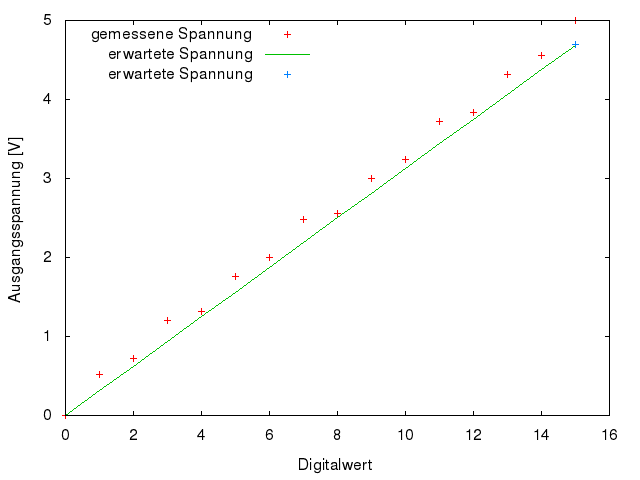
\includegraphics[width=\linewidth]{versuch9/versuch_9_1.png}
	\caption{Gemessene und erwartete Ausgangsspannung}
\end{figure}
Der Offsetfehler liegt bei 0V:
\begin{figure}[H]
	\centering
	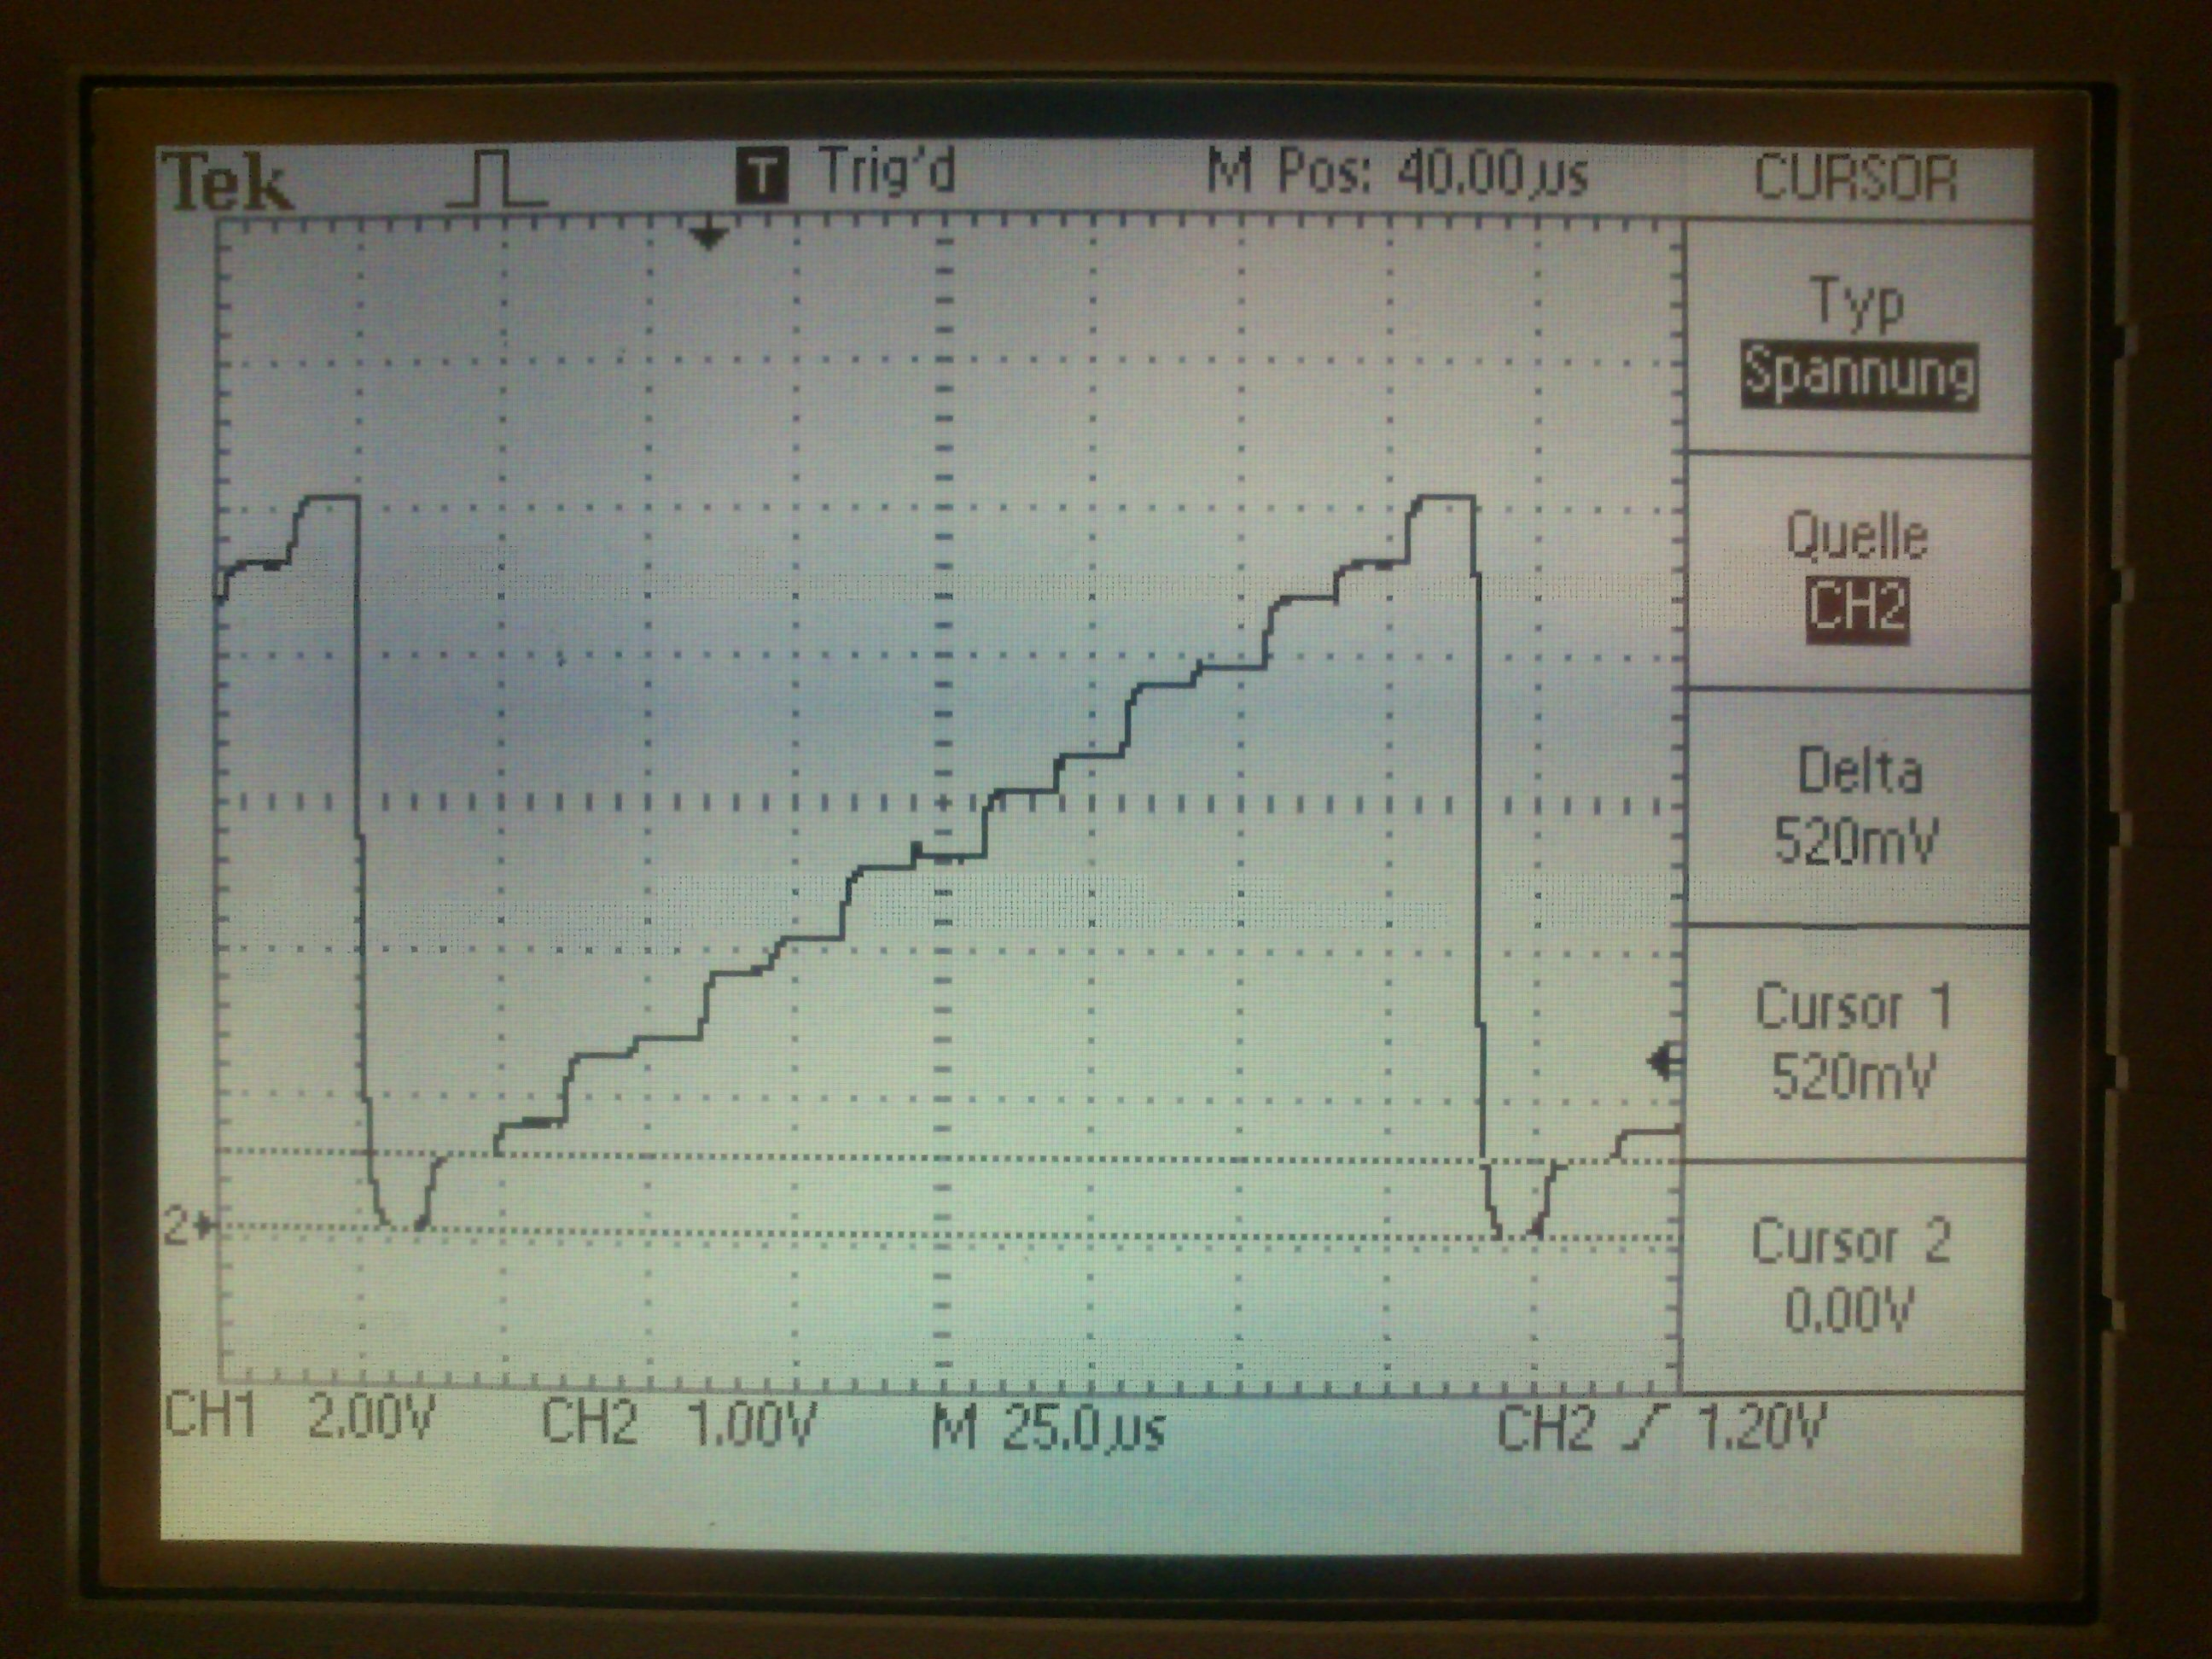
\includegraphics[width=\linewidth]{versuch9/oszi/DSC_0604.JPG}
	\caption{Wie man sieht, liegt die Spannung für 0b0000 bei 0V}
\end{figure}
Der Verstärkungsfehler beträgt $ 1.0667 = \frac{U_{out}(0b1111)_{real} - U_{offset}}{U_{out}(0b1111)_{erwartet}} = \frac{5V - 0V}{4.6875V} $

\subsection{Digitaler Sinusgenerator}
Ohne Kondensator ergab sich folgendes Bild:
\begin{figure}[H]
	\centering
	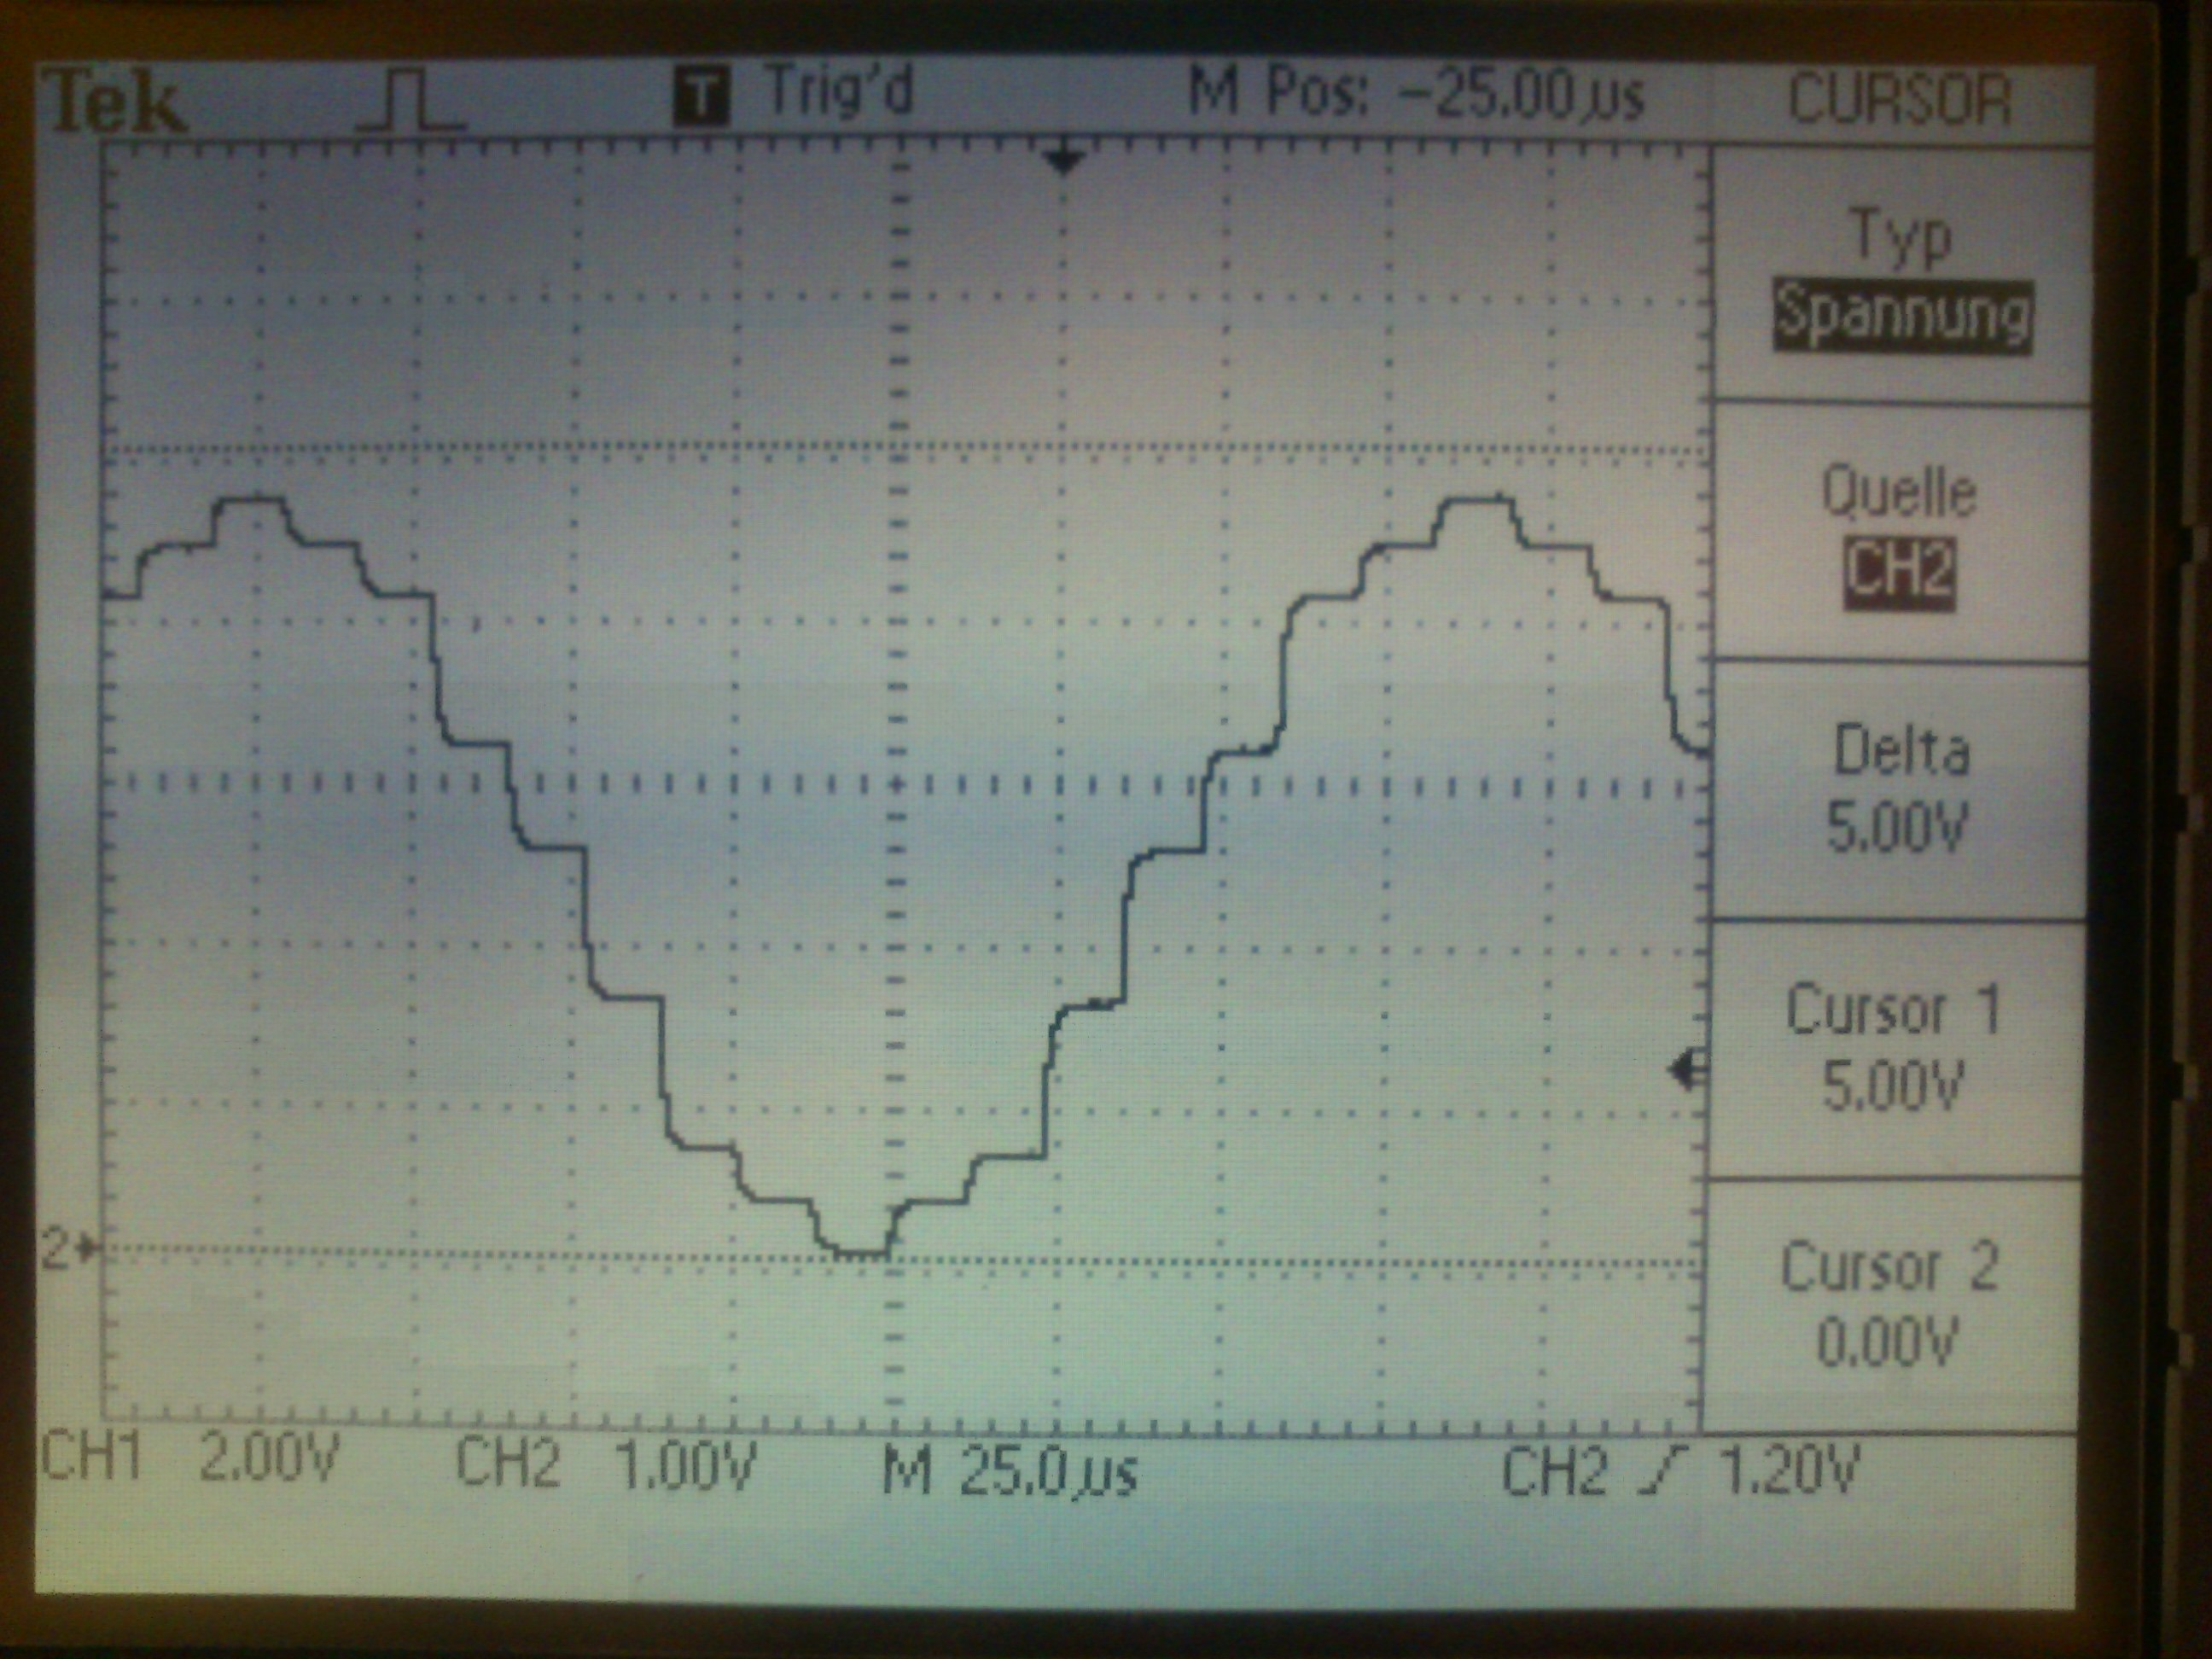
\includegraphics[width=\linewidth]{versuch9/oszi/DSC_0625.JPG}
	\caption{Sinusspannung ohne Tiefpass}
\end{figure}
\begin{figure}[H]
	\centering
	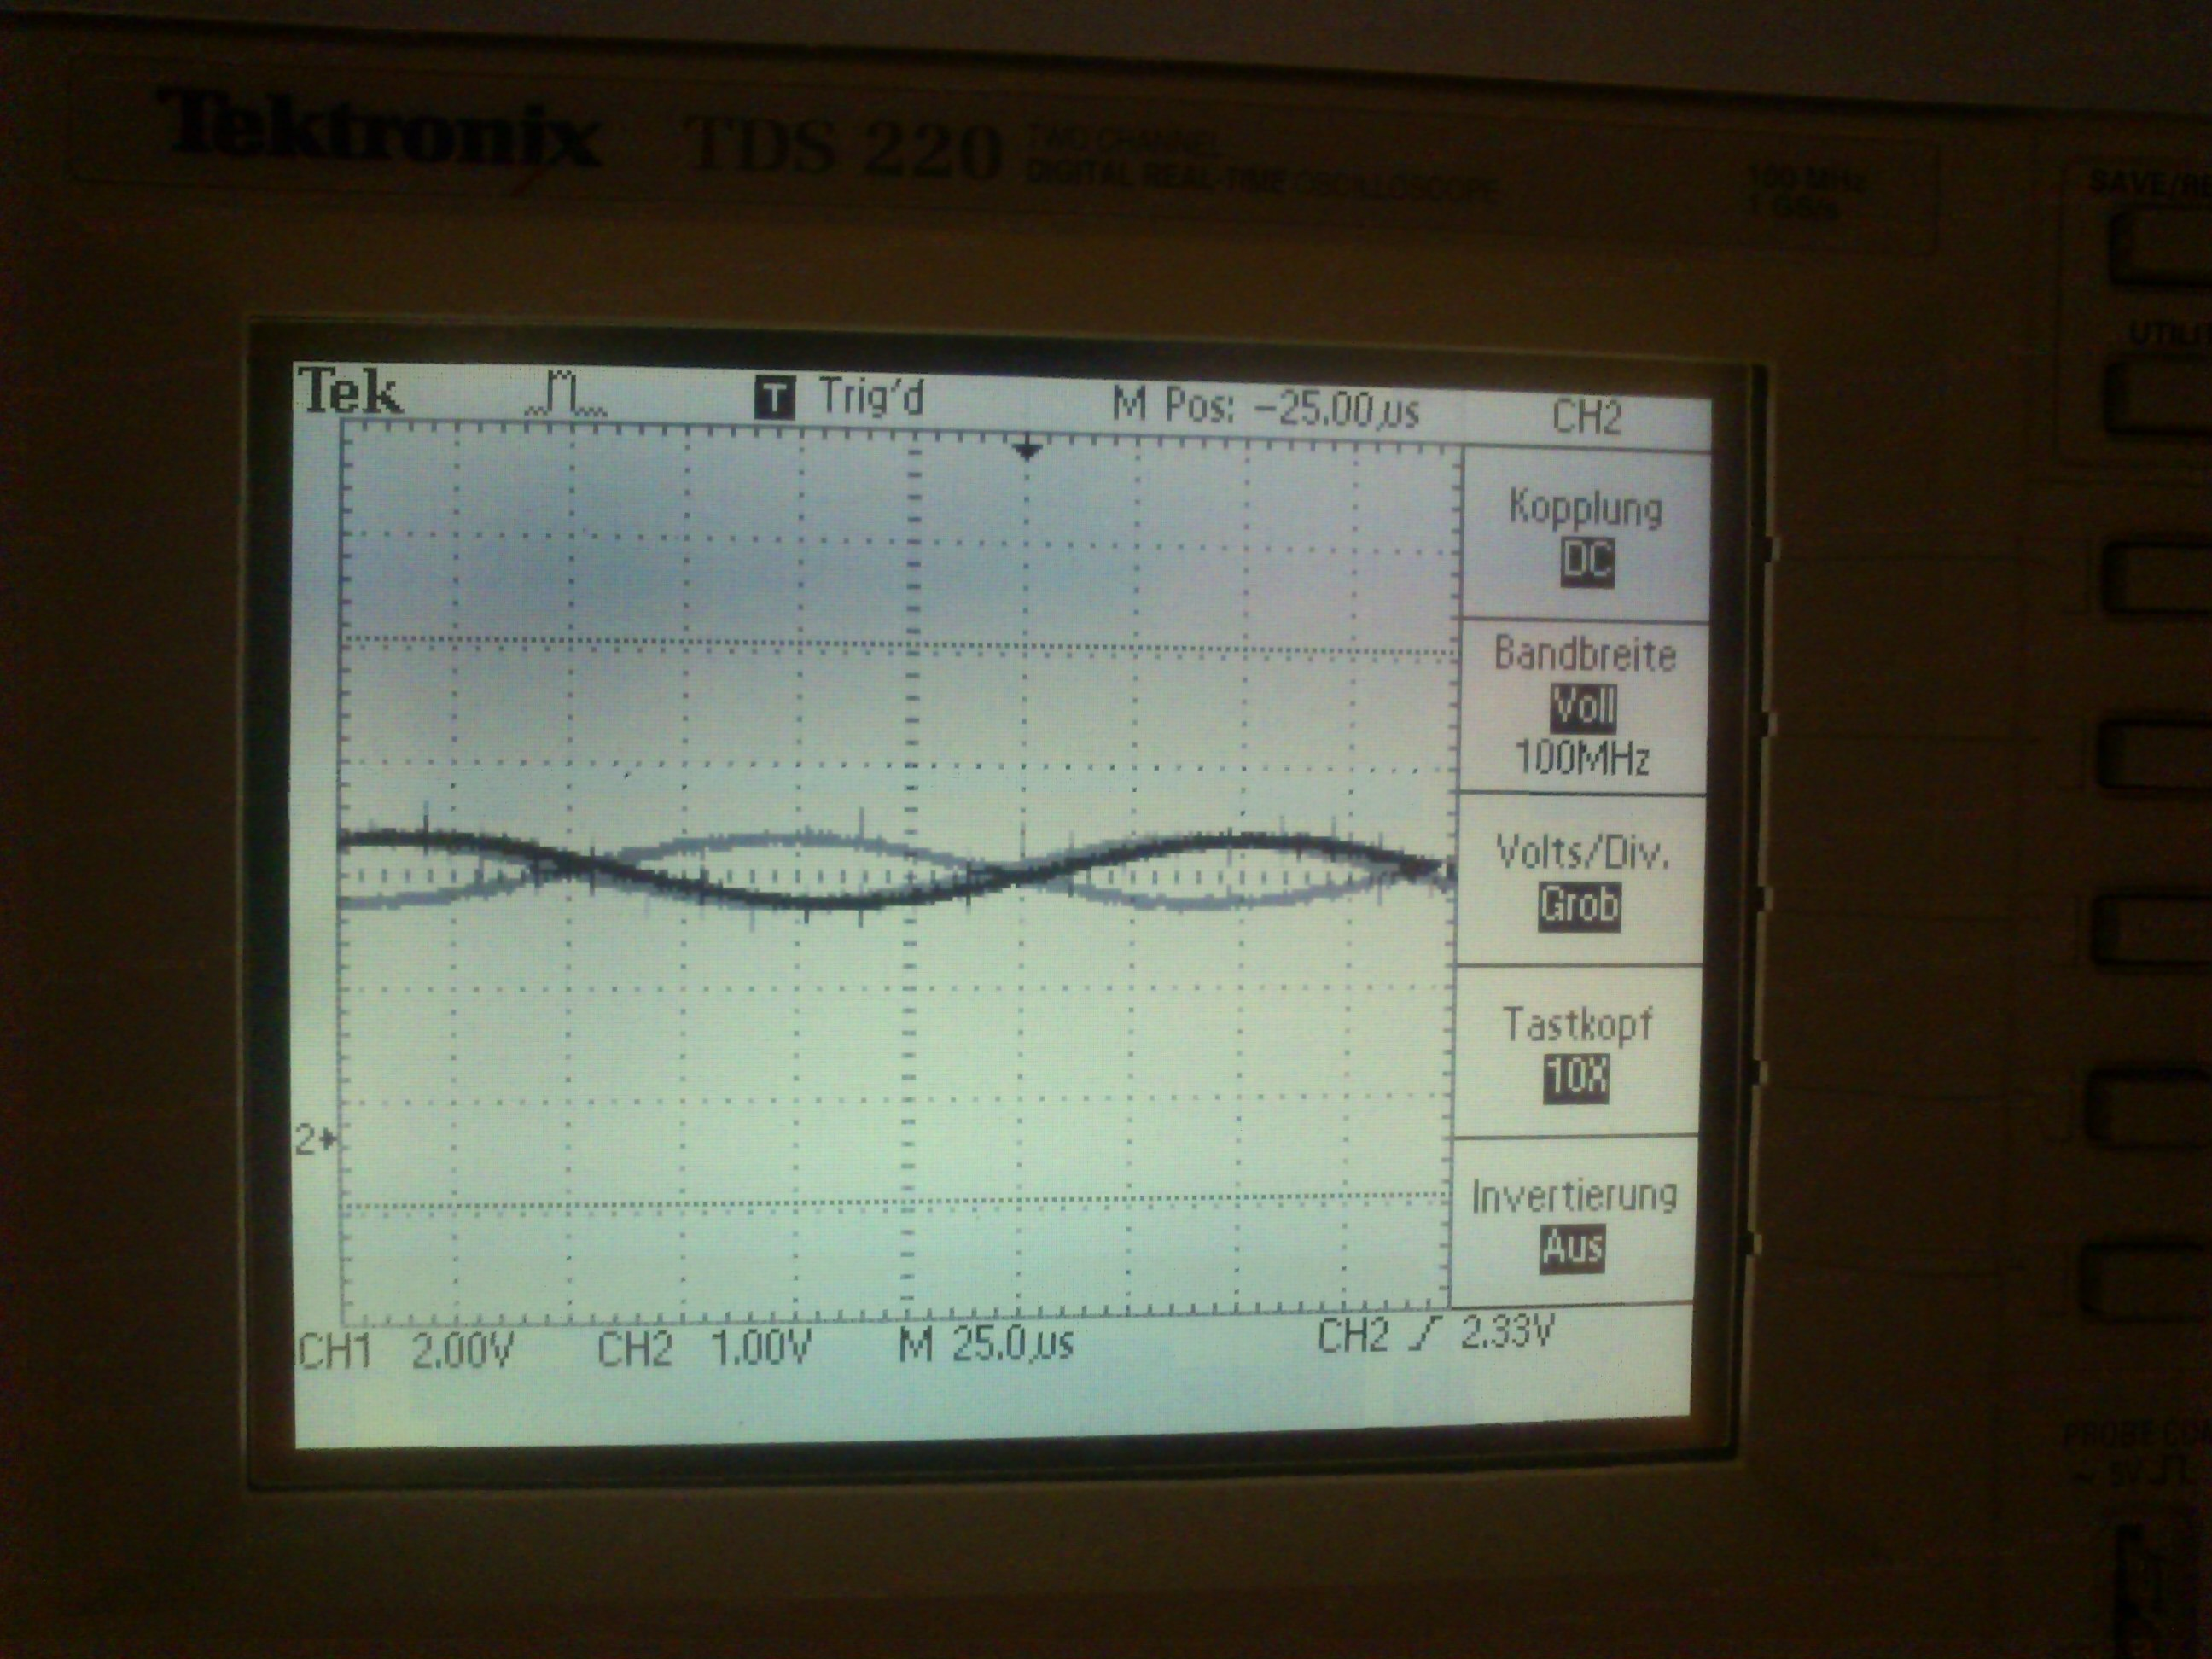
\includegraphics[width=\linewidth]{versuch9/oszi/DSC_0628.JPG}
	\caption{Der Kondensator ist eindeutig zu groß (4.7nF)}
\end{figure}
\begin{figure}[H]
	\centering
	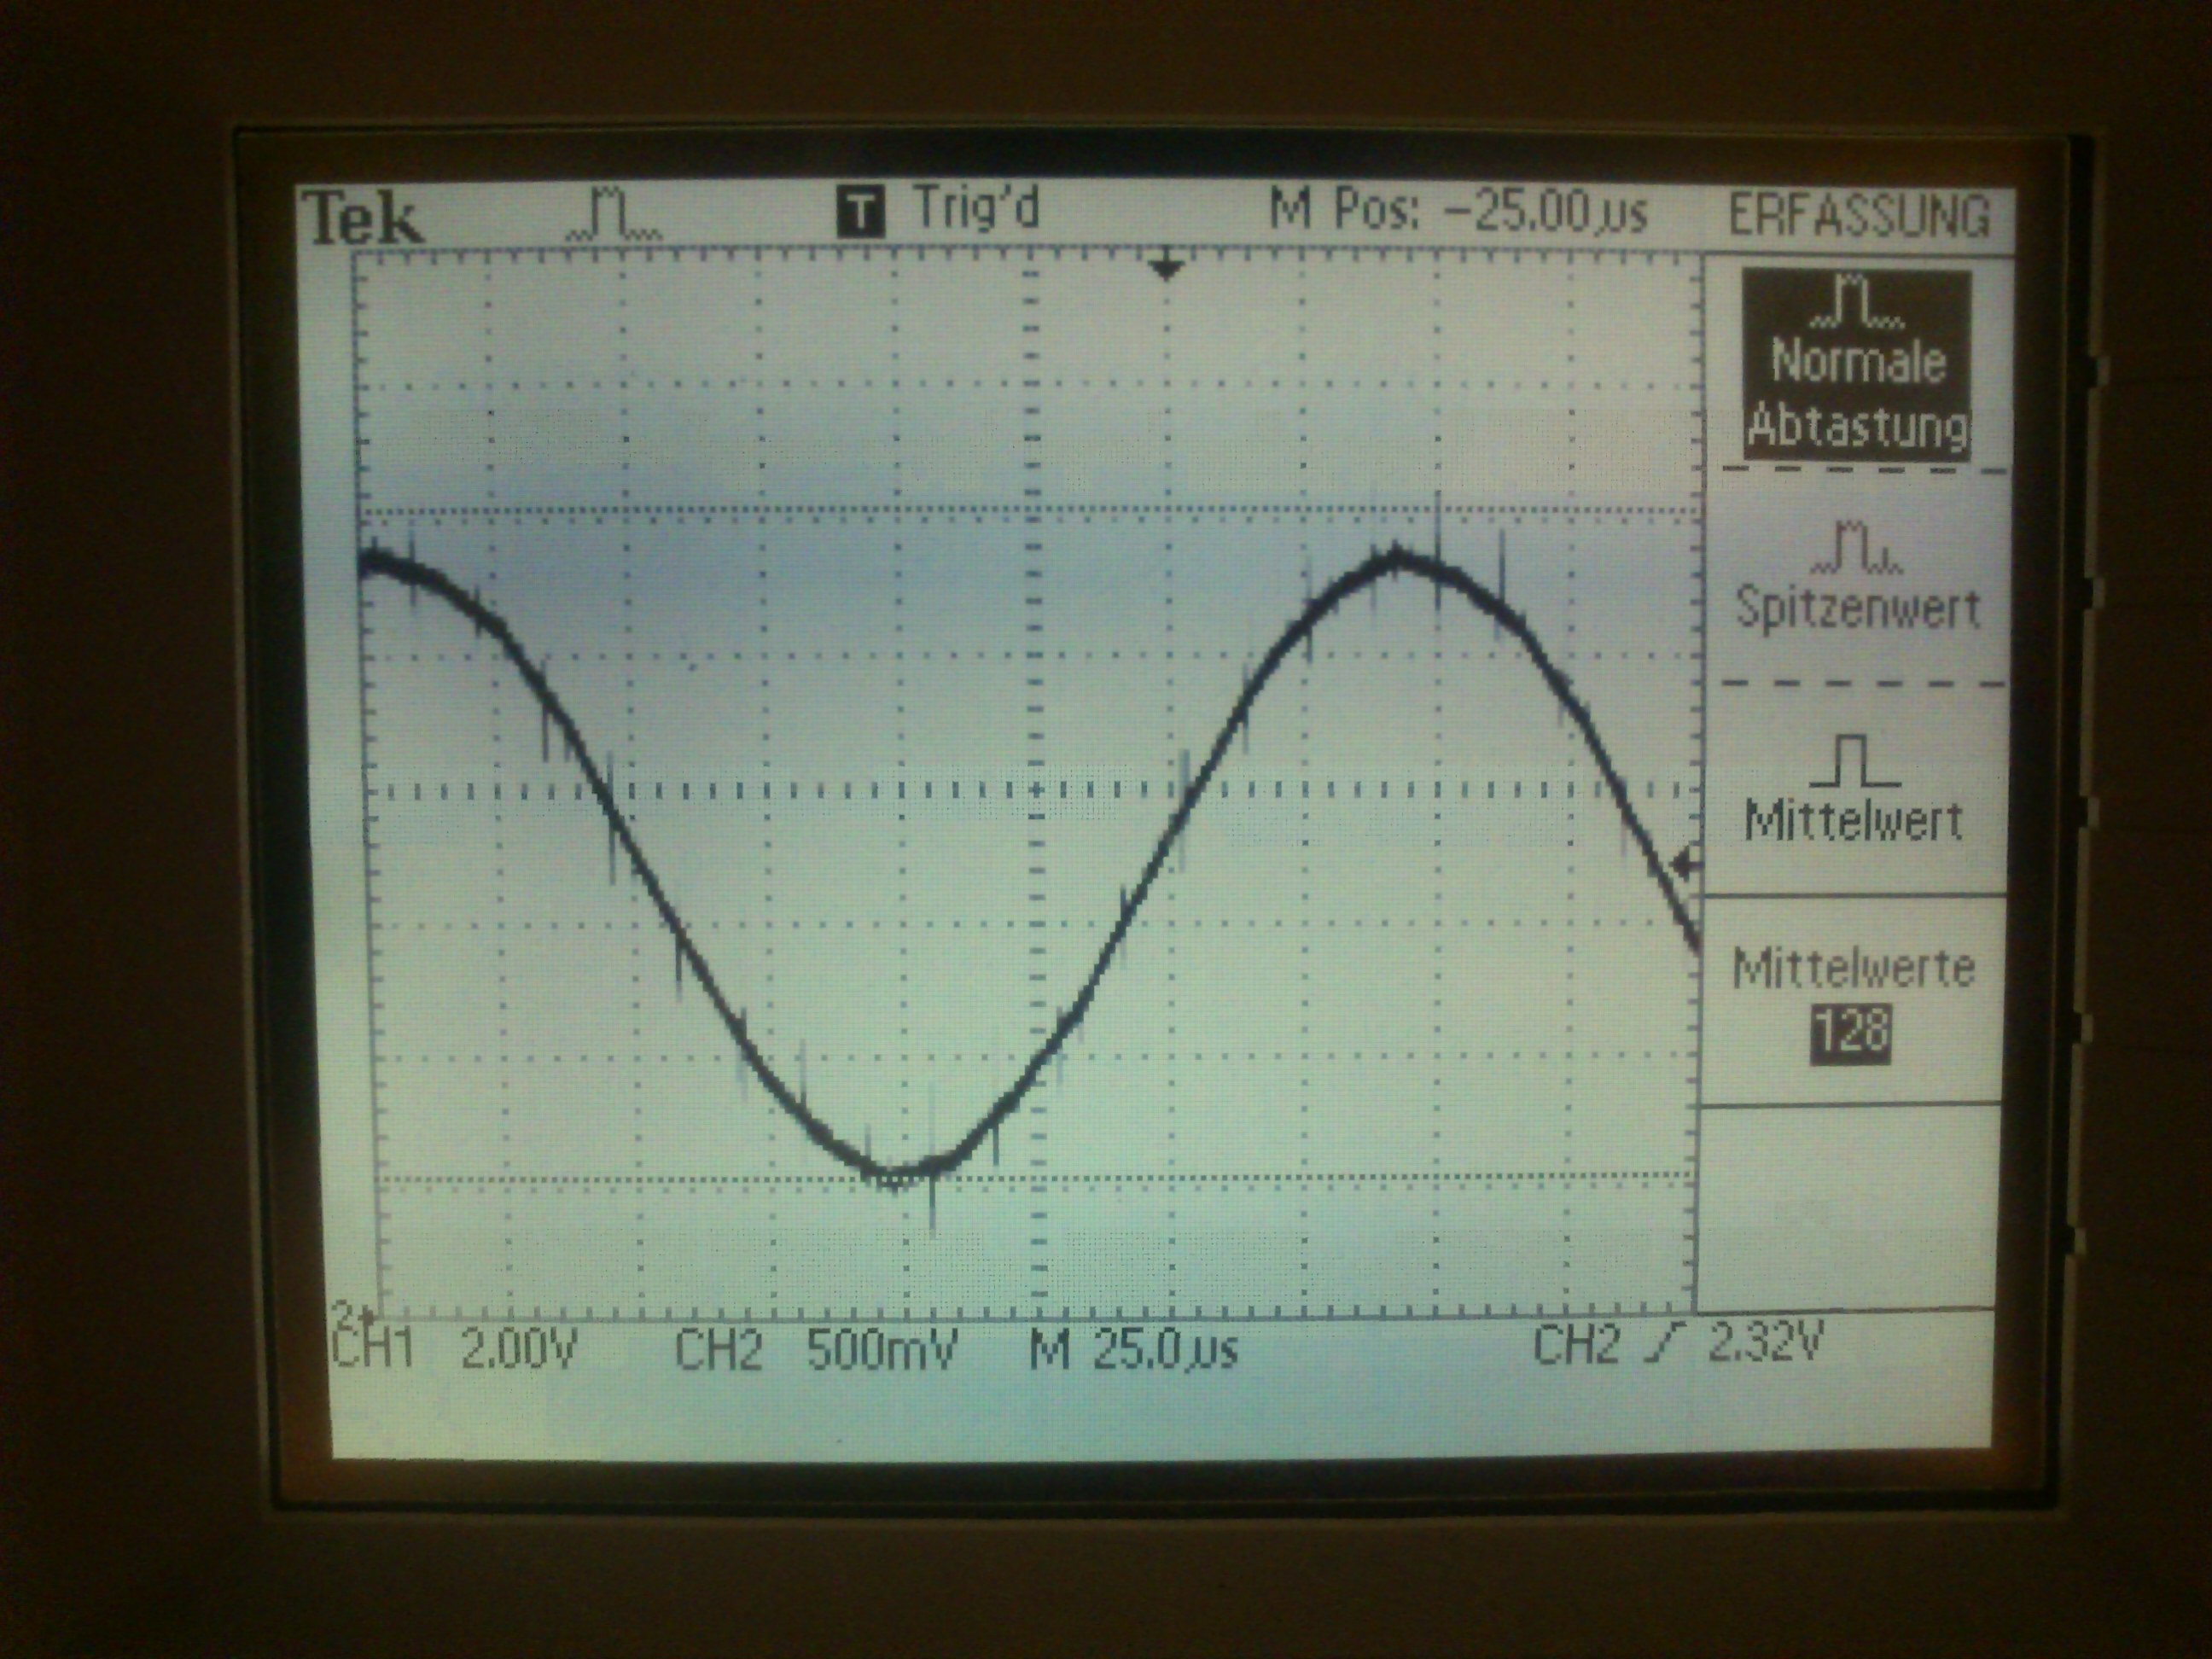
\includegraphics[width=\linewidth]{versuch9/oszi/DSC_0631.JPG}
	\caption{Sinusspannung mit einem passenden Kondensator (1.0nF)}
\end{figure}

\subsection{Aufbau eines ADCs nach dem Wägeverfahren}
Als erstes war der Widerstand R9 zu dimensioieren. Der Eingangsspannungsspannungsbereich sollte 0..1.5V betragen, somit müsste die Ausgangsspannung $U_{out}(0b1111)$ bei $0b1111 * \frac{1}{16} * 1.5 = 1.4062V$ betragen. Der Innenwiderstand des DAC von $R_i=50k\Ohm$ bildet mit $R_9$ einen Spannungsteiler. Somit ergibt sich:
\[U_{comp}=U_{out}(0b1111)*(R_9/(R_1+R_9))=1.4062V\]
\[\Rightarrow\; R_9=\frac{U_{comp}*R_i}{U_{out}(0b1111)*U_{comp}}=\frac{1.4062V*50k\Ohm}{4.6875-1.4062V}=21.427k\Ohm \]
Da in Serie zu $R_9$ noch ein Poti von 4.7k\Ohm verbaut wird, wählte ich den nächstkleineren verfügbaren Wert für $R_9$, 18k\Ohm.\\
R12 implementiert eine Hysterese und macht aus dem Komperator somit einen Schmitt-Trigger.

Als nächstes wurde die Kennlinie aufgenommen:
\begin{tabular}{ll}
	Spannung & Wert\\
	0.00V & 0b0000\\
	0.10V & 0b0001\\
	0.18V & 0b0010\\
	0.21V & 0b0011\\
	0.35V & 0b0100\\
	0.43V & 0b0101\\
	0.46V & 0b0110\\
	0.54V & 0b0111\\
	0.63V & 0b1000\\
	0.75V & 0b1001\\
	0.83V & 0b1010\\
	0.88V & 0b1011\\
	0.97V & 0b1100\\
	1.09V & 0b1101\\
	1.14V & 0b1110\\
	1.22V & 0b1111\\
\end{tabular}\\
Damit ergab sich folgendes Schaubild:
\begin{figure}[H]
	\centering
	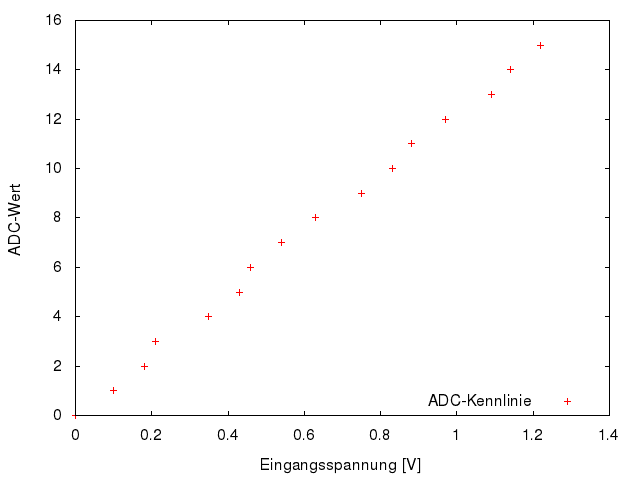
\includegraphics[width=\linewidth]{versuch9/versuch_9_3.png}
	\caption{Das ADC-Ergebnis als Plot}
\end{figure}
Leider habe ich im Eifer des Gefechts (und durch den im letzten Versuch vorhandenen Zeitdruck) vergessen, das Potentiometer einzustellen, daher rühren die schlechten Werte her. Die Nichtlinearität kann ich jedoch leider nicht erklären.

\subsection{Anzeige des kompletten "`Suchbaums"'}
\begin{figure}[H]
	\centering
	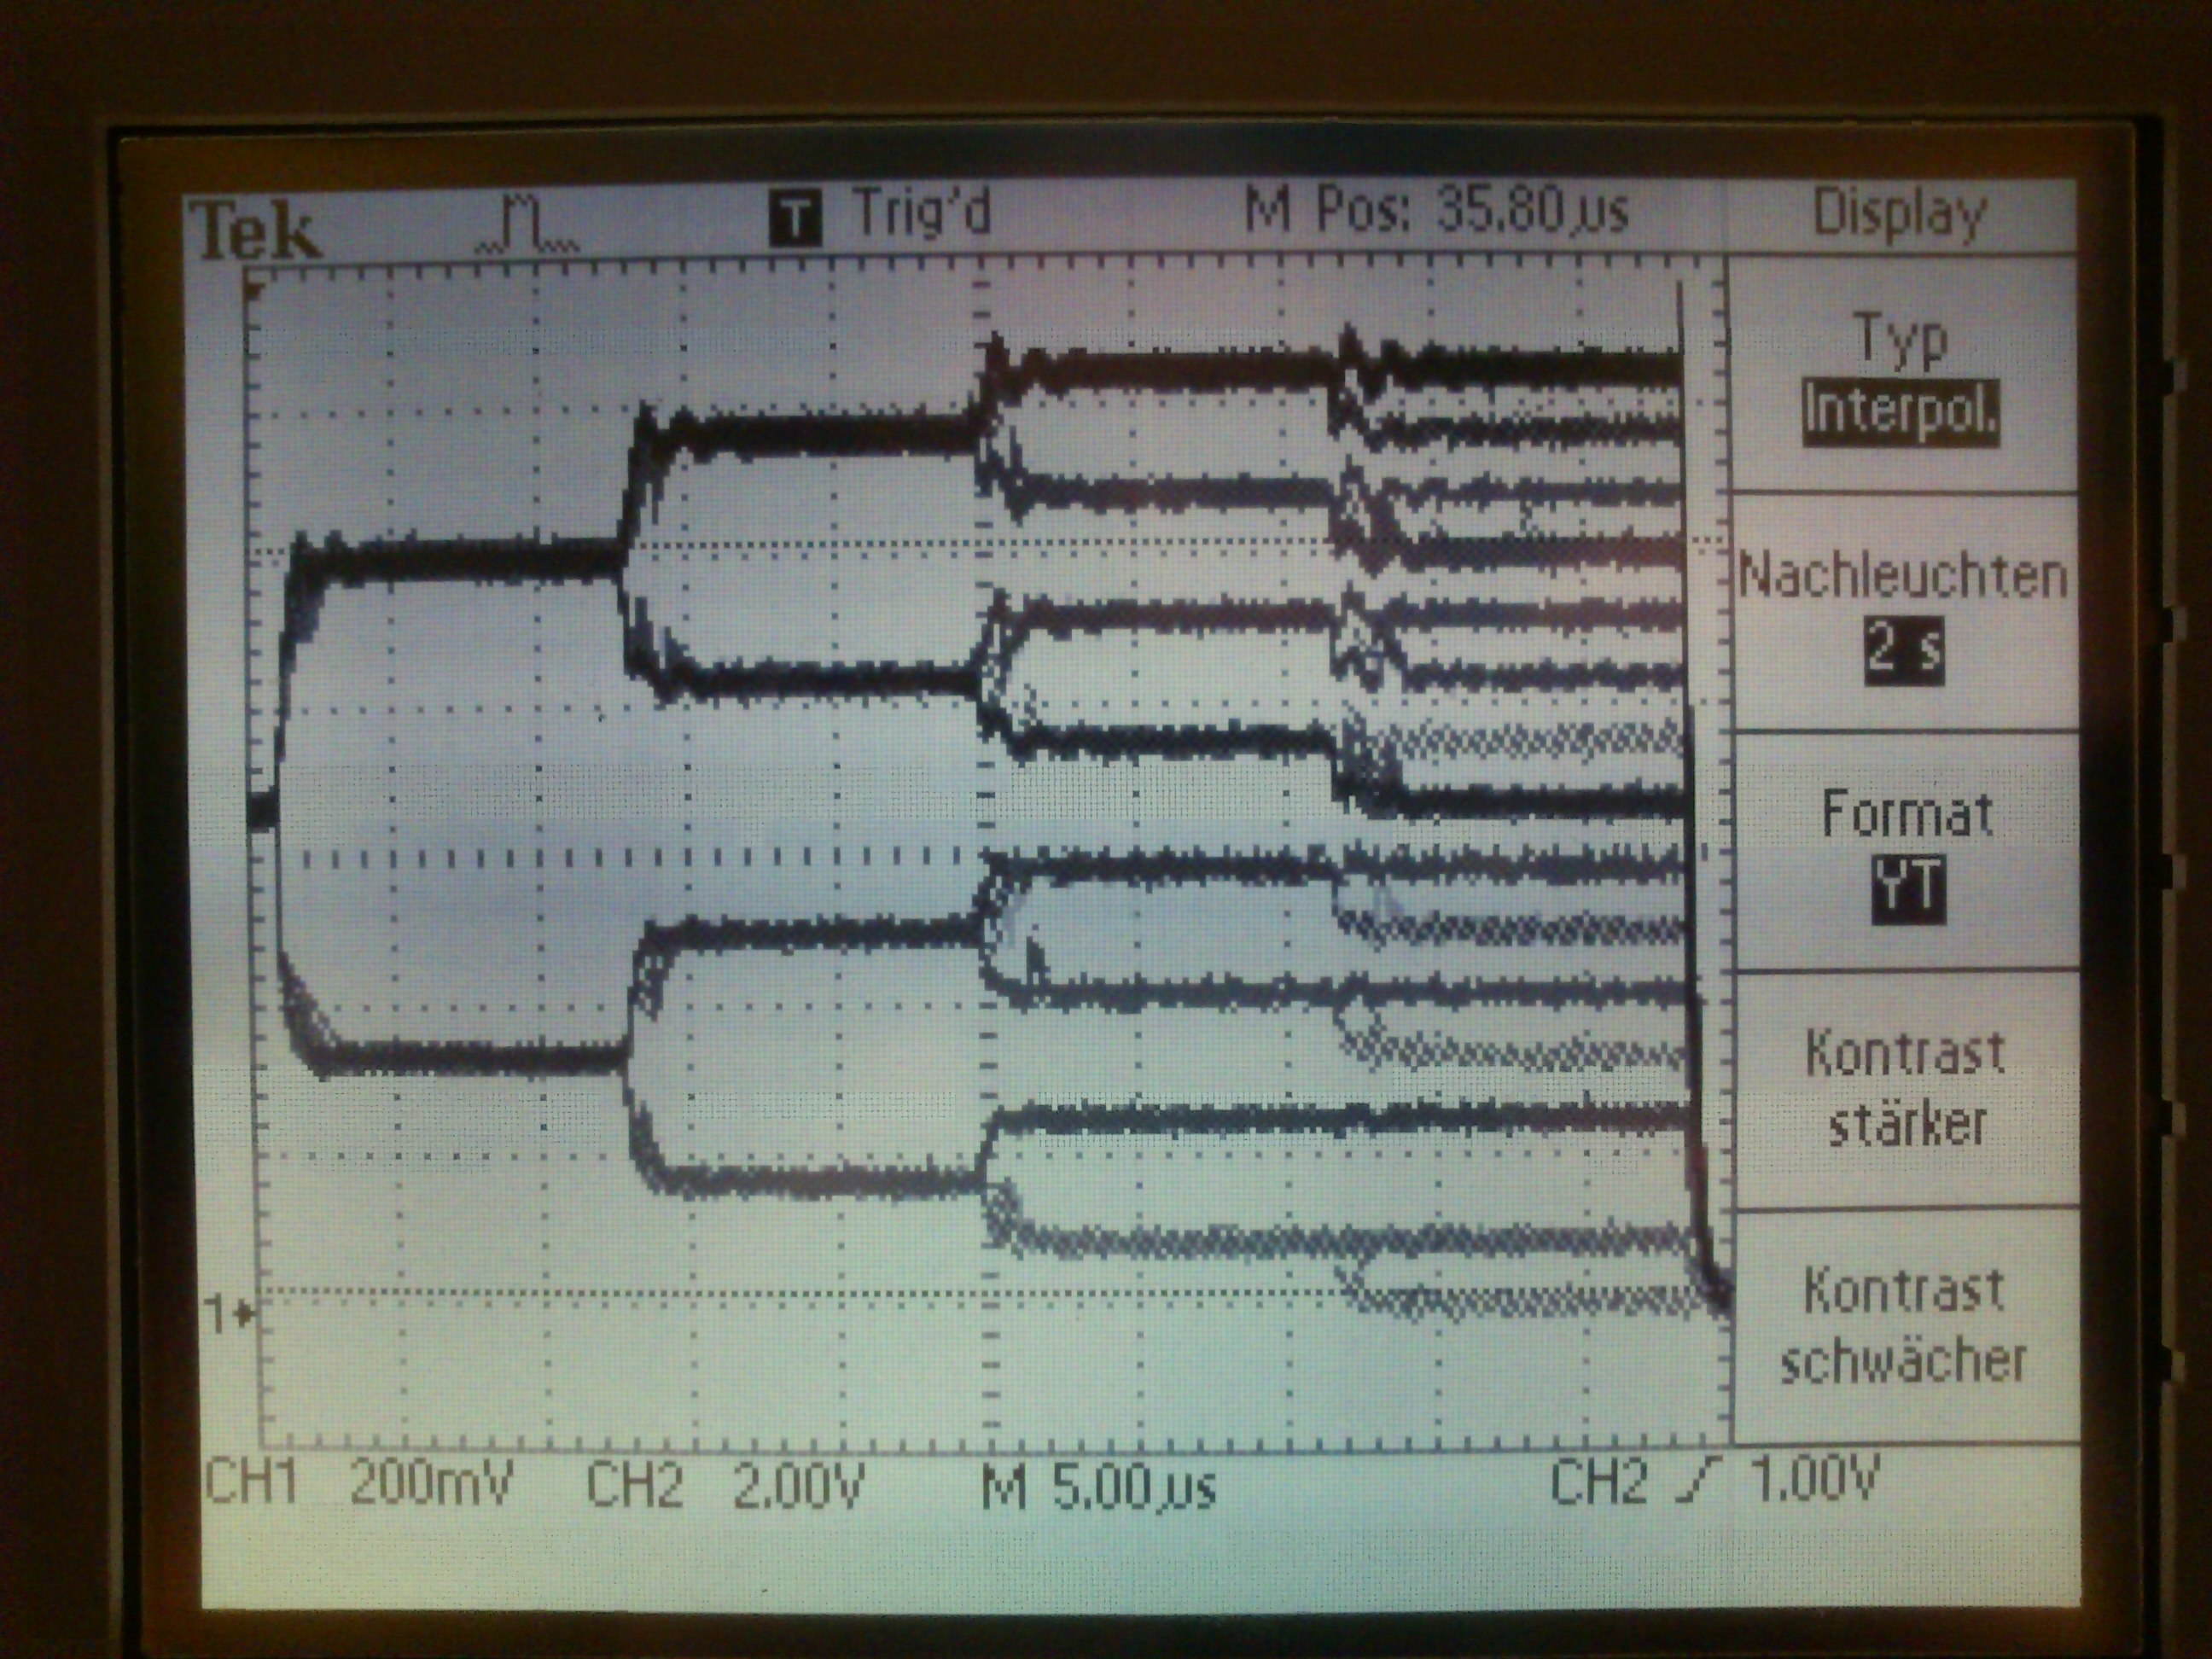
\includegraphics[width=\linewidth]{versuch9/oszi/DSC_0649.JPG}
	\caption{Der Suchbaum am Oszilloskop angezeigt}
\end{figure}

\subsection{Geschwindigkeit des Analog-Digital-Wandlers}
Es gilt:
\[t_{reg}=25 ns,\;t_{buf}=16 ns,\;t_{comp}=1,3 μs,\;t_{setup}=15 ns,\;t_{RC}=150ns\]
\[T_{Takt} = t_{reg}+t_{buf}+t_{comp}+t_{RC}=1491ns=1,491\µs\]
\[T_{Wandlung}=t_{setup}+4*T_{Takt}=5979ns=5,979\µs\]
\[\Rightarrow f_{Wandlung}=\frac{1}{T_{Wandlung}} = 167.25Hz\]
\[\Rightarrow f_{Eingang, max} = \frac{f_{Wandlung}}{2} = 83.625Hz\]

\subsection{LED-Anzeige}
Die Wahrheitstabelle des BCD-zu-7-Segment-Dekoders lässt sich einfach ablesen und sieht wie folgt aus:\\
\begin{tabular}{l|lllllll}
	Einganszahl [BCD] & a & b & c & d & e & f & g\\
	\hline
	0000	& 1 & 1 & 1 & 1 & 1 & 1 & 0\\
	0001	& 0 & 1 & 1 & 0 & 0 & 0 & 0\\
	0010	& 1 & 1 & 0 & 1 & 1 & 0 & 1\\
	0011	& 1 & 1 & 1 & 1 & 0 & 0 & 1\\
	0100	& 0 & 1 & 1 & 0 & 0 & 1 & 1\\
	0101	& 1 & 0 & 1 & 1 & 0 & 1 & 1\\
	0110	& 0 & 0 & 1 & 1 & 1 & 1 & 1\\
	0111	& 1 & 1 & 1 & 0 & 0 & 0 & 0\\
	1000	& 1 & 1 & 1 & 1 & 1 & 1 & 1\\
	1001	& 1 & 1 & 1 & 0 & 0 & 1 & 1\\
\end{tabular}
Die LED-Anzeige funktionierte ohne Probleme.

\subsection{Quantisierungsrauschen}
Unser Wandler hat eine Auflösung von 4 bit, also ist $U_{LSB}=0.093750V$. Somit ergibt sich $U_r^2$ zu $7.3242e-04 V^2$\\
Für $U_{1eff}^2$ ergibt sich $0.5*(16*0.093750V)^2/4=0.28125V^2$\\
Das Signal-Rausch-Verhältnis ergibt sich somit zu: $SNR [dB] = 10*\log \left(\frac{U_{1eff}^2}{U_r^2}\right) = 10*\log\left(\frac{0.28125V^2}{7.3242e-04 V^2}\right) db=25.843 dB$.

\vspace{2cm}
\Huge{ENDE}




